\documentclass[compress]{beamer}
\usepackage{natbib}
%\useoutertheme[footline=authorinstitutetitle]{miniframes}
%\usecolortheme{whale}
%\usecolortheme{orchid}
%\usetheme{CambridgeUS}
\usecolortheme{rose}
\useoutertheme{infolines}
\usefonttheme[onlymath]{serif}
%\setbeamertemplate{headline}[default]
\setbeamertemplate{headline}{
\begin{beamercolorbox}[ht=2.25ex,dp=2.75ex]{section in head/foot}
    \insertsectionnavigationhorizontal{\paperwidth}{}{\hfill}
\end{beamercolorbox}
}
\setbeamertemplate{footline}{
\leavevmode%
\hbox{%
\begin{beamercolorbox}[ht=2.25ex,dp=1ex,right]{date in head/foot}%
    \usebeamerfont{date in head/foot}\insertshortdate{}\hspace*{2em}
    \insertframenumber{} / \inserttotalframenumber\hspace*{2ex} 
\end{beamercolorbox}}%
\vskip0pt%
}
\usepackage{xcolor}
\setbeamertemplate{navigation symbols}{}
\mode<beamer>{\setbeamertemplate{blocks}[rounded][shadow=true]}
\setbeamercovered{transparent}
%\setbeamercolor{block body example}{fg=blue, bg=black!20}
%\setbeamercolor{title}{fg=darkgreen}
%\setbeamercolor{section}{fg=darkgreen}
%\setbeamercolor{subsection}{fg=darkgreen}




\usepackage{graphicx}
\usepackage{listings}
\usepackage{placeins}
\usepackage{hyperref}
\lstset{ 
    language=Python, % choose the language of the code
    basicstyle=\footnotesize\color{black},
    keywordstyle=\color{black}\bfseries, % style for keywords
    commentstyle=\color{blue},
	stringstyle=\color{magenta},
    numbers=none, % where to put the line-numbers
    numberstyle=\tiny, % the size of the fonts that are used for the line-numbers     
    backgroundcolor=\color{white},
    showspaces=false, % show spaces adding particular underscores
    showstringspaces=false, % underline spaces within strings
    showtabs=false, % show tabs within strings adding particular underscores
    frame=single, % adds a frame around the code
    tabsize=2, % sets default tabsize to 2 spaces
    rulesepcolor=\color{gray},
    rulecolor=\color{black},
    captionpos=b, % sets the caption-position to bottom
    breaklines=true, % sets automatic line breaking
    breakatwhitespace=false, 
}



\setbeamerfont{block title}{size={}}

\newcommand{\myurl}[1]{ { \footnotesize\textcolor{blue}{\url{#1}}  } }

\title{Software Quality and Sustainability Guidelines}
\subtitle{CLARIAH}
\author{Maarten van Gompel (RU), Reinier de Valk (DANS), Jauco Noordzij (Huygens), Andrea Scharnhorst (DANS)}
\date{October 7th, 2016}


\begin{document}

\begin{frame}
\maketitle
\end{frame}

\section{Introduction}

\begin{frame}{Introduction}


\begin{figure}

\includegraphics[height=7.5cm]{img/intro.jpg}
\end{figure}

\end{frame}

\begin{frame}{Introduction}

\begin{figure}

\includegraphics[height=6cm]{img/intro.jpg}
\end{figure}
\begin{center}
Software quality and sustainability should be an \textbf{essential component}
of the development process rather than an afterthought.
\end{center}
\end{frame}

\begin{frame}{Introduction}
    \begin{block}{Software plays an essential role}
        \begin{itemize}
            \item Development of advanced sofware is a core activity within CLARIAH.
            \item The CLARIAH infrastructure consists of numerous interconnected software components.
            \item The success of the whole depends on the success of its parts
        \end{itemize}
    \end{block}

    \begin{block}{Questions addressed}
        \begin{itemize}
            \item How do we ensure software is of good quality?
            \item ... How to measure this?
            \item ... What quality standards do we aim for?
            \item How do we ensure software is sustainable towards the future?
        \end{itemize}
    \end{block}

\end{frame}

\begin{frame}{Introduction}
    \begin{block}{Context}
        \begin{itemize}
        \item DANS \& eScience-NL report \citep{RESEARCHSOFTWARE}:
        \begin{itemize}
            \item Research software is a \textbf{fundamental component} of modern research.
            \item Software in academia \textbf{lags behind} commercial software.
            \item Pressure is on publication of new results: software is fragile
                and not sustainable or usable beyond project lifetime.
        \end{itemize}
        \item Research Software Sustainability: Report on Knowledge Exchange workshop
        \begin{itemize}
            \item Software is not data: software \textbf{must adapt} to the constant changes in its environment or will decay.
        \end{itemize}
        \item Software Sustainability Institute (UK): \url{http://software.ac.uk}
        \end{itemize}
    \end{block}
\end{frame}

\begin{frame}
    \begin{block}{Goals}
        \begin{enumerate}
            \item \textbf{Improve} software quality \& sustainability
            \item \textbf{Emphasise} the importance of good software development in academia
            \item \textbf{Provide practical guidelines} that allow developers and adopters to assess software on their own.
        \end{enumerate}
    \end{block}
    \begin{block}{Form}
        \begin{itemize}
            \item A \textbf{set of specific assessment criteria} grouped into various \textbf{dimensions}
            \item A web-based survey anybody can use to assess software: \url{http://softwarequality.clariah.nl}
            \item A list of minimal requirements for developers that offers a different perspective on the criteria.
        \end{itemize}
    \end{block}
\end{frame}

\section{Usage}

\begin{frame}{Usage of the guidelines}
    \begin{block}{How to use the guidelines?}
        For developers..
        \begin{itemize}
            \item self-assessment using the web-survey (\url{http://softwarequality.clariah.nl})
            \item add the survey results to your VC repository so others can see it
            \item provide us with feedback through our issue tracker!
                (\url{https://github.com/CLARIAH/software-quality-guidelines/issues})
        \end{itemize}
    \end{block}

    \begin{block}{Future}
        \begin{itemize}
            \item Revision of guidelines based on feedback after usage
            \item Incorporation of CLARIAH-specific interoperability criteria
            \item A software seal of approval?
        \end{itemize}
    \end{block}
\end{frame}

\section{Highlights}

\begin{frame}{Highlights}
\end{frame}

\begin{frame}{Accessibility: Version Control}
\begin{figure}
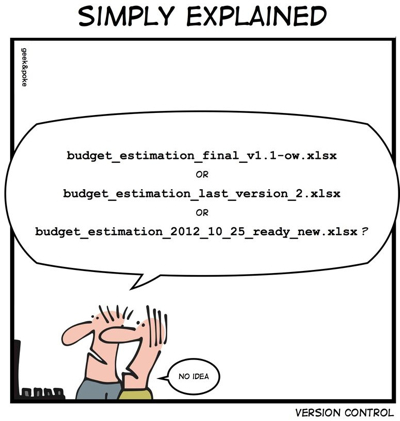
\includegraphics[height=7cm]{img/versioncontrol.jpg}
\end{figure}
\end{frame}

\begin{frame}{Accessibility: Version Control}
\begin{itemize}
    \item Always use \textbf{version control} for any software project
    \item Use \textbf{public} version control (e.g. Github) whenever possible
    \begin{itemize}
        \item increases project visibility/findability
        \item encourages contribution and interaction.
        \item provides infrastructure with issue trackers (bug reports), release management facilities
        \item transparency: allows users to assess the project's activity
        \item \url{https://github.com/CLARIAH}
    \end{itemize}
    \item Periodically publish releases of your software, using a sane version
        numbering scheme, accompanied with release notes or a changelog.
\end{itemize}
\end{frame}

\begin{frame}{Documentation}
\begin{figure}
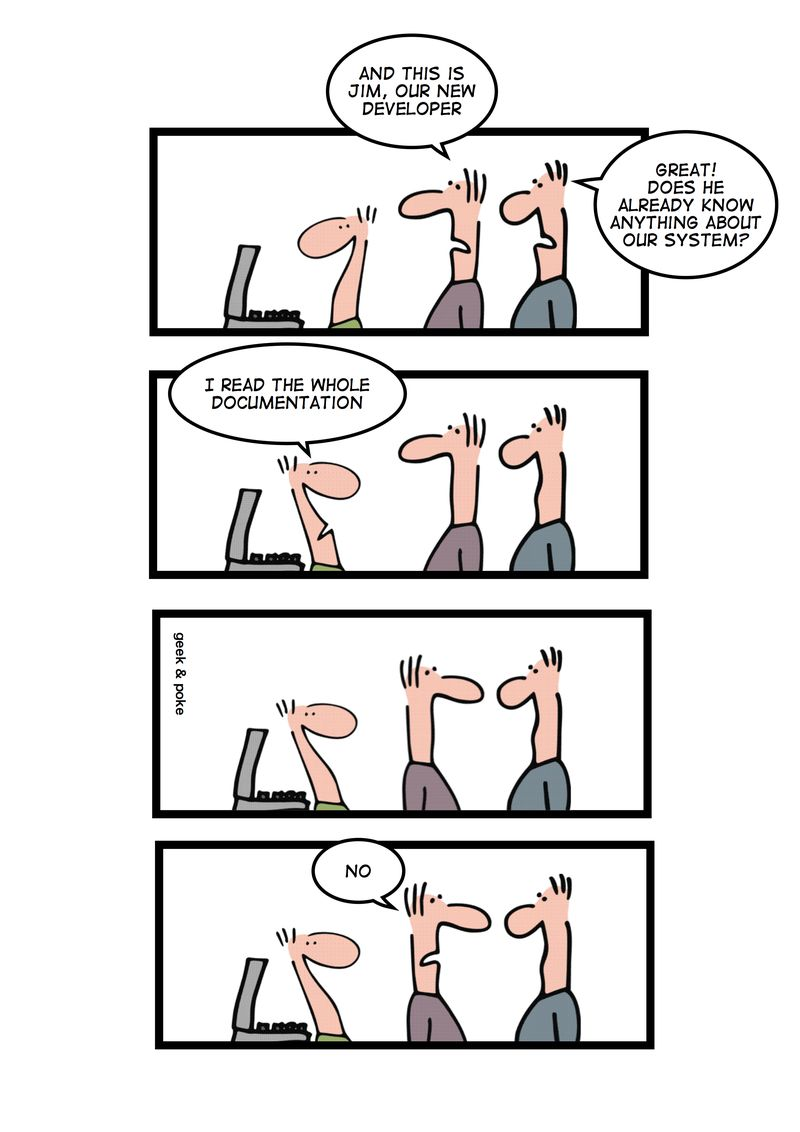
\includegraphics[height=8.3cm]{img/documentation.jpg}
\end{figure}
\end{frame}

\begin{frame}{Documentation}
\begin{itemize}
    \item Have a good and comprehensive \textbf{README} (plain-text) in your VC repository.
    \begin{itemize}
        \item \textbf{Tip:} Use Markdown or ReStructureText for mark-up
    \end{itemize}
    \item Document how to \textbf{build and install} the software
    \item Address \textbf{all the intended audiences} at the
        \textbf{appropriate levels}.
    \item Documentation should \textbf{live alongside the code} in the VC repository
    \item API documentation should be \textbf{automatically generated} from
        documentation comments in the source code \emph{(Doxygen, sphinx,
        javadoc)}
    \item Documentation should be up to date with the latest version.
    \item \textbf{Tip:} Have documentation auto-regenerate on every commit to
        your VC repo, using services like https://readthedocs.io
\end{itemize}
\end{frame}


\begin{frame}{Buildability \& Installability}
\begin{figure}
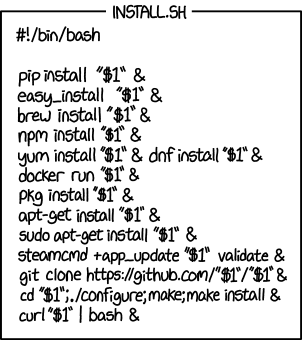
\includegraphics[height=7cm]{img/install.png}
\end{figure}
\end{frame}


\begin{frame}{Buildability \& Installability}
    \begin{itemize}
        \item There should be an automated build and install procedure for the software
            \emph{and all dependencies} on the target platform(s). Preferably
            through \textbf{one command}. 
        \item Use established build tools (GNU Autotools, CMake, Maven, Ant)
        \item Package and upload to the programming language's infrastructure to facilitate installation:
            \begin{itemize}
                \item Python - Python Package Index (http://pypi.org)
                \item Java - Maven (http://maven.org)
                \item Ruby - Gems (http://rubygems.org)
                \item Perl - CPAN (http://cpan.net)
                \item Javascript - npm
            \end{itemize}
        \item or  ...
    \end{itemize}
\end{frame}

\begin{frame}{Buildability \& Installability}
    \begin{itemize}
        \item Package and upload to the platform's repository to facilitate
            installation:
            \begin{itemize}
                \item Build packages for Linux distributions (DEB packages for
                        Debian/Ubuntu packages, Arch User Repository (AUR), RPM
                    for Fedora/CentOS/RHeL, etc)
                \item Consider Homebrew or macports for Mac, or the Mac App store.
                \item Apple's App store (iOS) Google's Play (Android) store for mobile apps.
            \end{itemize}        
        \item Last resort only: statically linked download archive from a project website
        \item Additionally, consider container or VM solutions (e.g, Docker, Vagrant, Ansible) for complex setups.
    \end{itemize}
\end{frame}

\begin{frame}{Testability}
\begin{figure}
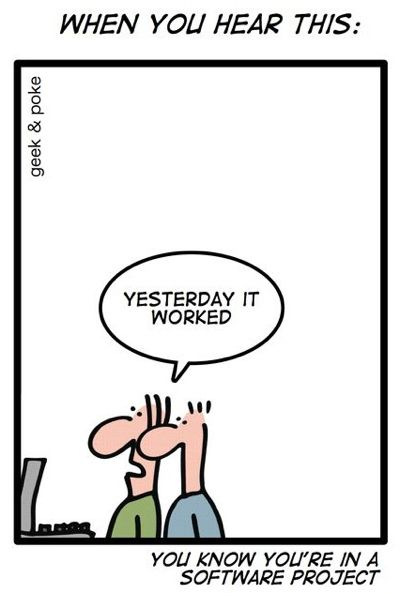
\includegraphics[height=8cm]{img/test3.jpg}
\end{figure}
\end{frame}

\begin{frame}{Testability}
    \begin{block}{Testability}
        \begin{itemize}
        \item If you didn't test it, it most likely doesn't work.
        \item Write automated tests (unit \& integration tests) for your software.
        \item Ensure automated tests cover all enough of your software.
        \item Use continuous integration platforms such as Travis-CI (https://travis-ci.org), Jenkins (http://jenkins.io) or others.
            \begin{itemize}
                \item These automatically run tests each time you commit code to your VC repo.
            \end{itemize}
        \end{itemize}
    \end{block}
\end{frame}

\begin{frame}{Community, Changeability \& Supportability}
\begin{figure}
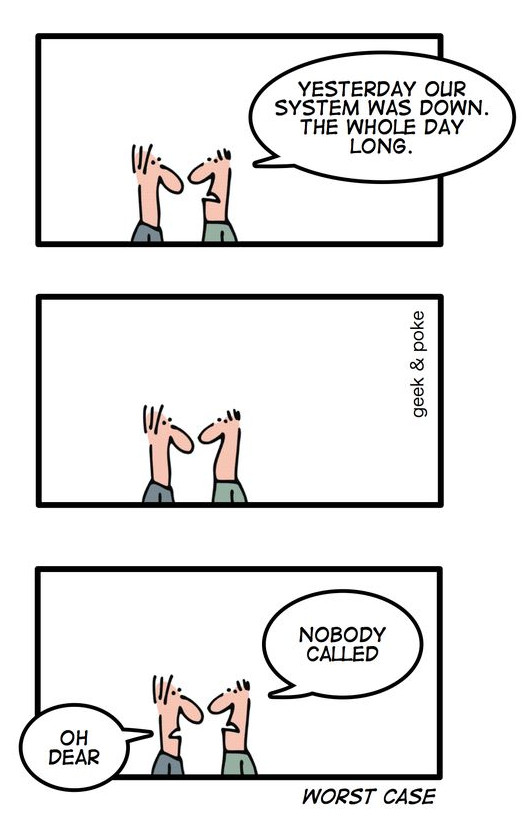
\includegraphics[height=8cm]{img/community.jpg}
\end{figure}
\end{frame}

\begin{frame}{Community, Changeability \& Supportability}
    \begin{block}{Community}
        \begin{itemize}
            \item Is the software used? Do you have usage statistics?
        \end{itemize}
    \end{block}
    \begin{block}{Changeability}
        \begin{itemize}
            \item Be open to outside contributors
            \item Code changes and authorships should be publicly visible through versioning control, with sane commit messages
            \item Is the software sufficiently backwards compatible?
        \end{itemize}
    \end{block}

    \begin{block}{Supportability}
        \begin{itemize}
            \item Be in touch with the users your software.
            \item Have a \textbf{public issue tracker} for tracking bugs and
                feature requests. Alternatively, have a mailing list
                (publically archived).
            \begin{itemize}
                \item Platforms like github provide an issue tracker automatically.
            \end{itemize}
        \end{itemize}
    \end{block}
\end{frame}

\begin{frame}{Analysability \& Reusability}
\begin{figure}
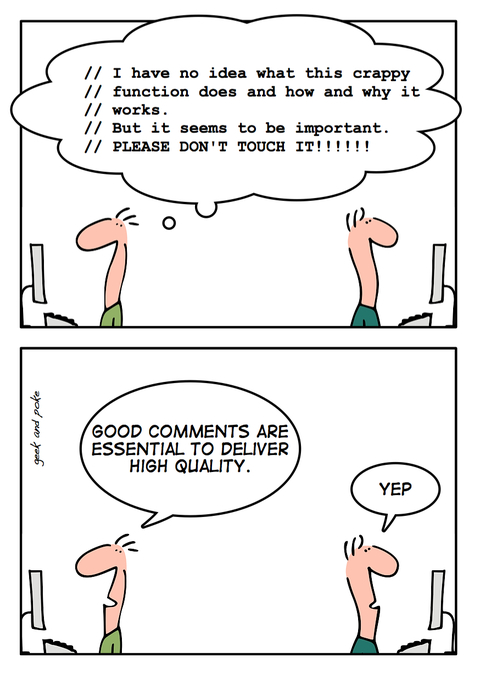
\includegraphics[height=8cm]{img/comments.jpg}
\end{figure}
\end{frame}

\begin{frame}{Analysability \& Reusability}

    \begin{block}{Analysability}
        \begin{itemize}
        \item Is the source code commented adequately?
        \item Is the source code cleanly laid out? (e.g. proper indentation)
        \item Are sensible named used?
        \item Follow established conventions for the programming language
        \end{itemize}
    \end{block}

    \begin{block}{Reusability}
        \begin{itemize}
            \item Does the software offer the \textbf{appropriate interfaces} for the
                respective audiiences? (command-line, web, GUI, API, web-api..)
            \item Is the software set up in a \textbf{modular} fashion?
            \begin{itemize}
                \item on \textbf{code level}: functions, classes
                \item abstraction of core logic from interfaces  (front-end/back-end separation)
                \item architectural: modules for different functionality
            \end{itemize}
        \end{itemize}
    \end{block}
\end{frame}

\begin{frame}{Security \& Privacy}
\begin{figure}
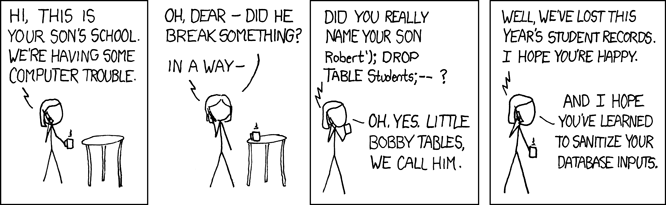
\includegraphics[width=12cm]{img/bobbytables.png}
\end{figure}
\end{frame}

\begin{frame}{Security \& Privacy}

    \begin{block}{Security}
        \begin{itemize}
            \item Validate user input
            \item Be aware of possible attack vectors:
            \begin{itemize}
                \item DB injection in e.g. SQL queries
                \item shell injection (when invoking system calls)
                \item cross-site request forgery
                \item denial of service
            \end{itemize}
            \item Do not rely on outdated platforms or libraries 
            \item Never run anything as root
        \end{itemize}
    \end{block}
    \begin{block}{Privacy}
        \begin{itemize}
            \item Never store unhashed passwords
            \item Require authentication to access sensitive user data
        \end{itemize}
    \end{block}

\end{frame}


\begin{frame}
\begin{center}

\Large{Questions?}

\vspace{1cm}

\emph{Comics by}: Geek \& Poke and XKCD


\end{center}

\end{frame}



\section{References}

\begin{frame}
\footnotesize
\bibliographystyle{apalike}
\bibliography{../softwareguidelines}
\end{frame}

\section{Extra}

\begin{frame}{Extra: Dimensions (1/2)}
    \begin{block}{Usability Dimensions}
        \begin{itemize}    
            \item \textbf{Understandability} - Is the software easily understood? 
            \item \textbf{Documentation} -- Comprehensive well-structured documentation?
            \item \textbf{Buildability}  -- Straightforward to build from source on a supported system?
            \item \textbf{Installability} -- Straightforward to install and deploy on a supported system?
            \item \textbf{Learnability} -- Easy/intuitive to learn how to use its functions?
        \end{itemize}
    \end{block}
    \begin{block}{Sustainability \& Manageability Dimensions}
        \begin{itemize}    
            \item \textbf{Identity} -- Project/software identity is clear and unique? 
            \item \textbf{Copyright} -- Licencing and ownership Adoption of appropriate open-source license
            \item ...
        \end{itemize}
    \end{block}
\end{frame}

\begin{frame}{Extra: Dimensions (2/2)}
    \begin{block}{Sustainability \& Manageability Dimensions}
        \begin{itemize}    
            \item \textbf{Community} -- Evidence of current/future community
            \item \textbf{Accessibility} -- Good facilities to obtain versions of the software?
            \item \textbf{Testability} -- Easy to verify if the software functions correctly?
            \item \textbf{Portability} -- Usable on multiple platforms?
            \item \textbf{Supportability} -- Evidence of current/future developer support?
            \item \textbf{Analysability} -- Easy to understand at the source-code level?
            \item \textbf{Changeability} -- Easy to modify and contribute changes? 
            \item \textbf{Performance} -- Resource demands/consumption
            \item \textbf{Interoperability} 
            \item \textbf{Security \& Privacy}
        \end{itemize}
    \end{block}
\end{frame}
\end{document}

